\problemname{Kiki Boba}
\noindent
``\texttt{Kiki}'' and ``\texttt{boba}'' form a fascinating sound-symbolic connection, where people spontaneously associate sharp sounds like ``\texttt{kiki}'' 
with jagged shapes and softer sounds like ``\texttt{boba}'' with rounder shapes. 
This reveals an underlying link between sounds and visual properties, 
providing insight into how our brains intuitively create meaning and associations.

Fergus has long held a keen interest in phonetics, and based on this sound-symbolic connection, he has developed a theory! 
He believes that all words can be categorized into 4 categories. In other words, each word is either a word corresponding to the 
figure on the left, like ``\texttt{kiki}'', or a word corresponding to the figure on the right, like ``\texttt{boba}'', or a word 
that is a combination of both, or a word that is none of the aforementioned alternatives.

\begin{figure}[h]
  \centering
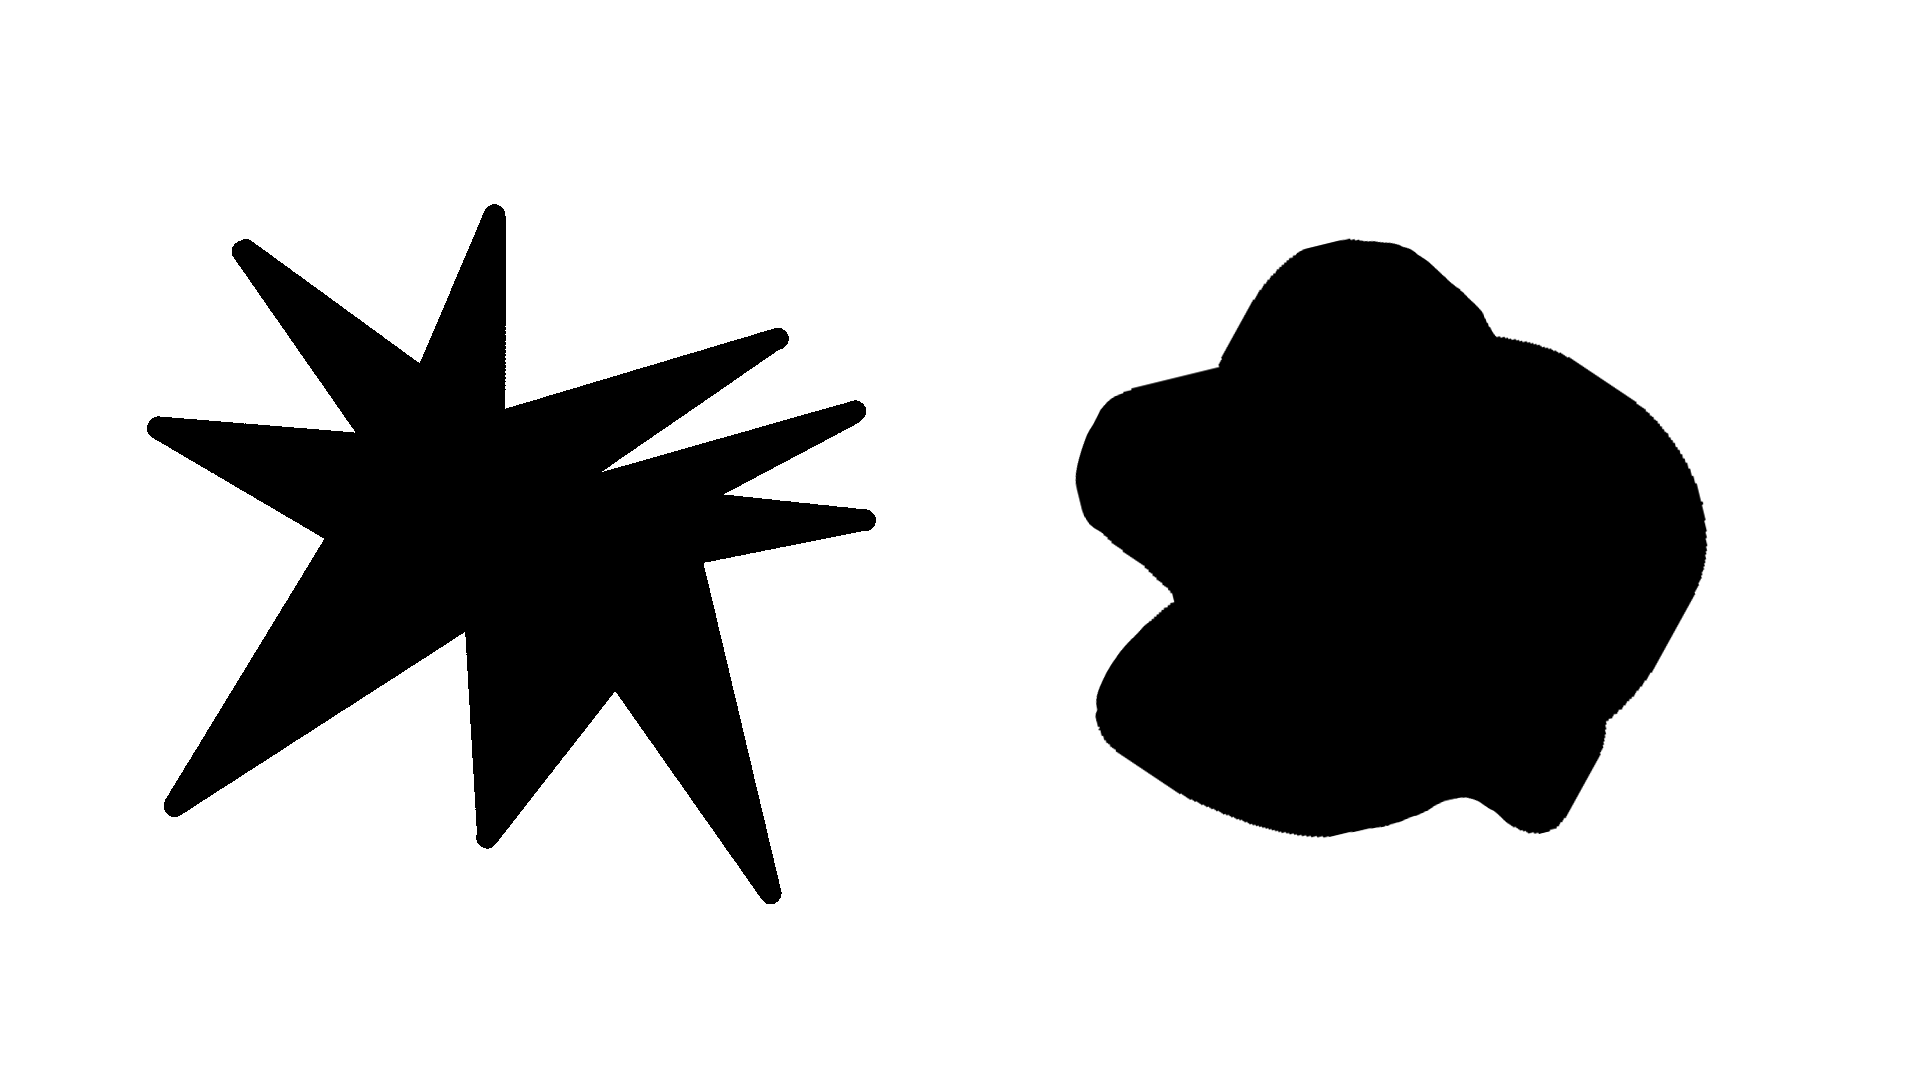
\includegraphics[width=0.6\textwidth]{kikiboba.png}
  \caption{Figure to the left is commonly associated with "kiki". Figure to the right is commonly associated with "boba".}
  \label{fig:kikiboba}
\end{figure}

Fergus determines that a word belongs to a category according to the following rules:
If there are more ``\texttt{b}'' than ``\texttt{k}'' in the word, then the word is a ``\texttt{boba}'' word.
If there are more ``\texttt{k}'' than ``\texttt{b}'' in the word, then the word is a ``\texttt{kiki}'' word.
If the word contains an equal number of ``\texttt{b}'' and ``\texttt{k}'', then Fergus calls it a ``\texttt{boki}'' word.
These rules hold with one exception:
If there are no ``\texttt{b}'' and ``\texttt{k}'' in the word, the word is neither close to a ``\texttt{boba}'' word nor a ``\texttt{kiki}'' word. In this case, Fergus refers to the word as a ``\texttt{none}'' word.

Help Fergus write a program that, given a word, can categorize the word according to Fergus' rules.

\section*{Input}
The only line of the input contains a string consisting of characters ``\texttt{a}''-``\texttt{z}'', the word that Fergus wants to categorize.

\section*{Output}
Print a category: either ``\texttt{boba}'', ``\texttt{kiki}'', ``\texttt{boki}'' or ``\texttt{none}'', according to Fergus' rules stated above.
There is always one category that fits each word.

\section*{Points}
Your solution will be tested on several test case groups.
To get the points for a group, it must pass all the test cases in the group.

\noindent
\begin{tabular}{| l | l | p{12cm} |}
  \hline
  \textbf{Group} & \textbf{Point value} & \textbf{Constraints} \\ \hline
  $1$    & $20$       & The word is only one character long. \\ \hline
  $2$    & $50$       & The word has atleast one of either ``\texttt{k}'' or ``\texttt{b}'', but never both at the same time. \\ \hline
  $3$    & $30$       & No additional constraints. \\ \hline
\end{tabular}

\section*{Explanation of sample 1}
The word contains 2 ``\texttt{b}'', while there are none of ``\texttt{k}''. In other words there are more of ``\texttt{b}'' than ``\texttt{k}'', which means that the answer is ``\texttt{boba}''.

\section*{Explanation of sample 3}
The word contains 1 ``\texttt{b}'' and 1 ``\texttt{k}''. There are an equal number of ``\texttt{b}'' and ``\texttt{k}'', which means the answer is ``\texttt{boki}''.
